%%%%%%%%%%%%%%%%%%%%%%%%%%%%%%%%%%%%%%%%%
% LaTeX Template
% Version 1.4 (15/5/16)
%
% This template has been downloaded from:
% http://www.LaTeXTemplates.com
%
% Original author:
% Frits Wenneker (http://www.howtotex.com) with extensive modifications by
% Vel (vel@LaTeXTemplates.com)
%
% License:
% CC BY-NC-SA 3.0 (http://creativecommons.org/licenses/by-nc-sa/3.0/)
%
%%%%%%%%%%%%%%%%%%%%%%%%%%%%%%%%%%%%%%%%%

%----------------------------------------------------------------------------------------
%	PACKAGES AND OTHER DOCUMENT CONFIGURATIONS
%----------------------------------------------------------------------------------------

\documentclass[twoside,twocolumn]{article}

\usepackage{blindtext} % Package to generate dummy text throughout this template 

\usepackage[sc]{mathpazo} % Use the Palatino font
\usepackage[T1]{fontenc} % Use 8-bit encoding that has 256 glyphs
\linespread{1.05} % Line spacing - Palatino needs more space between lines
\usepackage{microtype} % Slightly tweak font spacing for aesthetics

\usepackage[english]{babel} % Language hyphenation and typographical rules

\usepackage[hmarginratio=1:1,top=32mm,columnsep=20pt]{geometry} % Document margins
\usepackage[hang, small,labelfont=bf,up,textfont=it,up]{caption} % Custom captions under/above floats in tables or figures
\usepackage{booktabs} % Horizontal rules in tables

\usepackage{lettrine} % The lettrine is the first enlarged letter at the beginning of the text

\usepackage{enumitem} % Customized lists
\setlist[itemize]{noitemsep} % Make itemize lists more compact

\usepackage{abstract} % Allows abstract customization
\renewcommand{\abstractnamefont}{\normalfont\bfseries} % Set the "Abstract" text to bold
\renewcommand{\abstracttextfont}{\normalfont\small\itshape} % Set the abstract itself to small italic text

\usepackage{titlesec} % Allows customization of titles
\renewcommand\thesection{\Roman{section}} % Roman numerals for the sections
\renewcommand\thesubsection{\roman{subsection}} % roman numerals for subsections
\titleformat{\section}[block]{\large\scshape\centering}{\thesection.}{1em}{} % Change the look of the section titles
\titleformat{\subsection}[block]{\large}{\thesubsection.}{1em}{} % Change the look of the section titles

\usepackage{fancyhdr} % Headers and footers
\pagestyle{fancy} % All pages have headers and footers
\fancyhead{} % Blank out the default header
\fancyfoot{} % Blank out the default footer
\fancyhead[C]{Harvey Hughes $\bullet$ February 2019 $\bullet$ Emmanuel College} % Custom header text
\fancyfoot[RO,LE]{\thepage} % Custom footer text

\usepackage{titling} % Customizing the title section

\usepackage{hyperref} % For hyperlinks in the PDF

\usepackage{graphicx}
\graphicspath{ {images/} }

\newenvironment{reusefigure}[2][htbp]
  {\addtocounter{figure}{-1}%
   \renewcommand{\theHfigure}{dupe-fig}% If you're using hyperref
   \renewcommand{\thefigure}{\ref{#2}}% Figure counter is \ref
   \renewcommand{\addcontentsline}[3]{}% Avoid placing figure in LoF
   \begin{figure}[#1]}
  {\end{figure}}
\usepackage{wrapfig}
\usepackage{amsmath}
\usepackage{xcolor}
\usepackage{listings}

%----------------------------------------------------------------------------------------
%	TITLE SECTION
%----------------------------------------------------------------------------------------

\setlength{\droptitle}{-4\baselineskip} % Move the title up

\pretitle{\begin{center}\Huge\bfseries} % Article title formatting
\posttitle{\end{center}} % Article title closing formatting
\title{3F8 - Inference } % Article title
\author{%
\\
\textsc{Harvey Hughes} \\
\normalsize Emmanuel College \\ % Your institution
\normalsize Lab Date : 13/2/19 \\
\normalsize \href{mailto:hh458@cam.ac.uk}{hh458@cam.ac.uk} % Your email address
}
\date{\today} % Leave empty to omit a date
\renewcommand{\maketitlehookd}{%
\begin{abstract}
\noindent
hghjdgjhdghjdsghfhdghdfh
\newline
\end{abstract}
}

%----------------------------------------------------------------------------------------

\begin{document}

% Print the title
\maketitle

%----------------------------------------------------------------------------------------
%	ARTICLE CONTENTS
%----------------------------------------------------------------------------------------

\section{Introduction}

\lettrine[nindent=0em,lines=3]{D}uring the course of this lab several classification techniques were used to identify the two classes in the dataset shown in figure \ref{fig:1}. The performance of each classifier is measured by testing on an unseen test dataset once training has been completed. The classifiers used were a linear logistic function and non linear radial basis functions.

\begin{figure}[h]
  \centering
    \includegraphics[width=\linewidth]{1-Data}
  \caption{The datasets to be classified}
  \label{fig:1}
\end{figure}
%------------------------------------------------
\section{1. Preparation exercises}
The classification aims to maximise the likelihood of the data by optimising the weights, $\beta$. For this the log-likelihood: $\mathcal{L}(\beta )=logP(y|X,\beta ))$ is maximised. This is a non trivial optimisation problem therefore gradient ascent is used. This involves an initial guess at $\beta$ values then updating in the direction that increases log-likelihood. See equations \ref{update} and \ref{grad} for the form of this process. 

\begin{equation}
\label{update}
\beta^{(new)}=\beta^{(old)}+\eta \frac{\partial \mathcal{L}}{\partial \beta}\bigg\rvert_{\beta^{(old})}
\end{equation}

Where $\eta$ is a hyper-parameter called the leaning rate. A low value for $\eta$ is likely to cause slow convergence to the maxima, however a high value is often worse as it leads to oscillations about the maxima or never reaching it. Therefore, $\eta$ needs to be chosen carefully often by trialling a few values.

\begin{equation}
\label{grad}
\begin{split}
&\frac{\partial \mathcal{L}}{\partial \beta} = \sum^N_{n=1}y_n(1-\sigma(\beta^T\tilde{x}^{(n)}))\tilde{x}^{(n)} \\
&\sigma(\beta^T\tilde{x}^{(n)}) = \frac{1}{1+exp(-\beta^T\tilde{x}^{(n)})}\\
\end{split}
\end{equation}

$\tilde{x}^{(n)}$ in the linear classifier is equal to ($x^{(n)}$,1) in order to handle biases, therefore $\beta$ is a (3,1) vector of weights.
The implementation of this gradient ascent method used a vectorised form of the parameters to increase speed. This can be seen in appendix 1.1.
%--------------------------------------------------------------
\section{2. Linear Model}
Initially a linear model for separating the data groups was investigated. The data groups aren't in distinct groups that can be separated by one linear line see figure \ref{} therefore a linear model won't be very successful. 
\subsection{Training}
Using 80\% of the available data the linear model was trained using gradient ascent. 100 iterations were run with $neta =0.001$, the convergence to maximum log-likelihood can be seen in figure \ref{fig:T1}. After training $\beta= (-0.108,0.904,0.338)^T$

\begin{figure}[h]
  \centering
    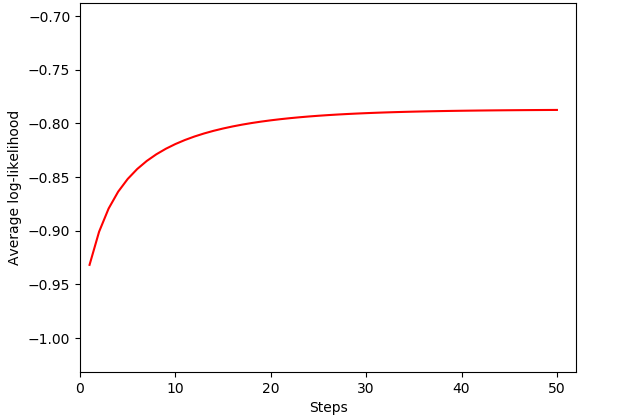
\includegraphics[width=\linewidth]{linearlog}
  \caption{Log-Likelihood being maximised for the linear model}
  \label{fig:T1}
\end{figure}

%------------------------------------------------

%------------------------------------------------
\subsection{Probability contours}
in order to visualise the classification process probability contours can be drawn on the data set. these indicate the probability of a certain $(x_1,x_2)$ residing in the blue class. Figure \ref{fig:C1} shows these contours. It's easily seen here that the accuracy of a linear classifier won't be too high on the data set due to the mixed clusters of each class in the dataset.

\begin{figure}[h]
  \centering
    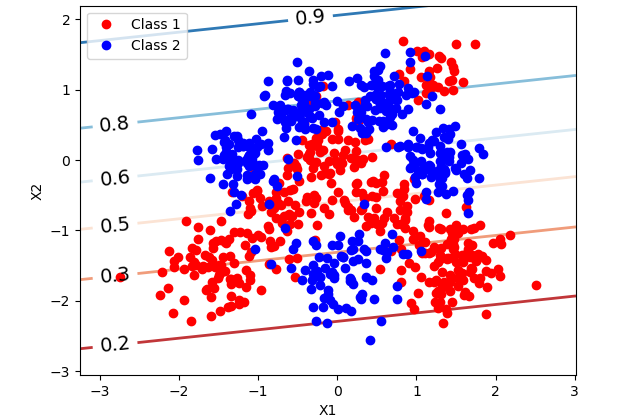
\includegraphics[width=\linewidth]{linearcontour}
  \caption{Probability contours of residing in the blue class for the linear model}
  \label{fig:C1}
\end{figure}

%------------------------------------------------
\subsection{Confusion Matrix}
To analyse the accuracy of classification more precisely a confusion matrix can be calculated. The confusion matrix is calculated using the unseen test set based on the optimum weights previously found. The on diagonal terms represent correctly classifying the data point, and off diagonal terms are incorrect classifications. The code for computing $\mathcal{C}$ is shown in the appendix 1.2.
\newline 

\begin{center}
$\mathcal{C}=  
\begin{bmatrix}
    0.35 & 0.155  \\
    0.18 & 0.315 \\
\end{bmatrix}$
\newline
\end{center}

The confusion matrix shows that 66.5\% of the test data was correctly classified.

%------------------------------------------------

%--------------------------------------------------------------
\section{3. Radial basis functions}
To improve classification accuracy non-linear techniques need to be used. This is done through the use of radial basis functions shown in equation \ref{rbf}

\begin{equation}
\label{rbf}
\tilde{x}_{m+1}^{(n)} = exp (\frac{-1}{2l^2}\sum^2_{d=1} (x_d^{(n)} - x_d^{(m)})^2)
\end{equation}

 The result of this is extra inputs in $\tilde{x}^{(n})$ which are 2D quadratics (radial basis functions) centred on each training data point with a certain width l. These extra inputs allow the model to classify using non linear regions meaning separate clusters can be identified and therefore reducing the error. The widths being tests are l =[1, 0.1, 0.01].
\subsection{Training}
Once again 80\% of the data was used to train on in order to find the optimum value for the extended (800,1) weight vector. Figures \ref{fig:T2} - \ref{fig:T4} show the training progress across iterations. 

\begin{figure}[h]
  \centering
    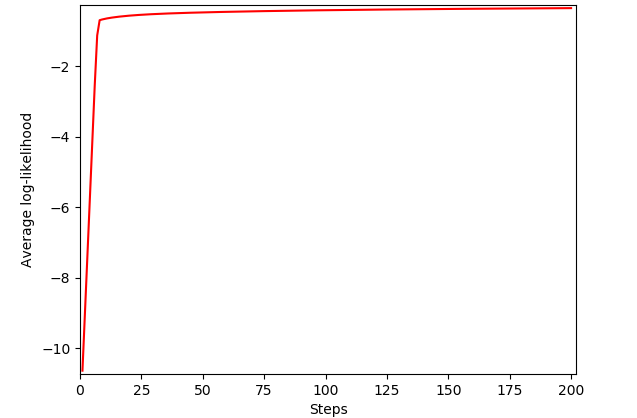
\includegraphics[width=\linewidth]{l=1log}
  \caption{Log-Likelihood being maximised when l=1}
  \label{fig:T2}
\end{figure}
\begin{figure}[h]
  \centering
    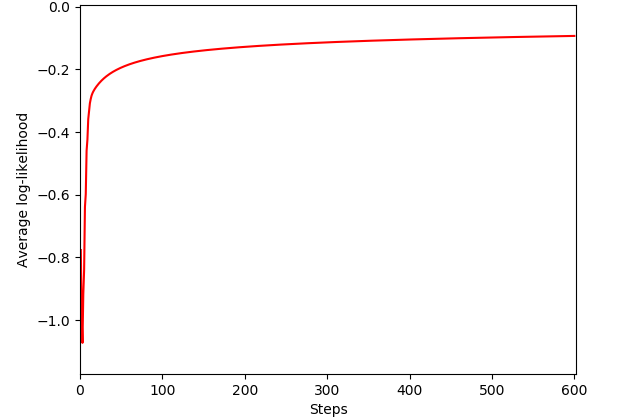
\includegraphics[width=\linewidth]{l=0-1log}
  \caption{Log-Likelihood being maximised when l=0.1}
  \label{fig:T3}
\end{figure}
\begin{figure}[h]
  \centering
    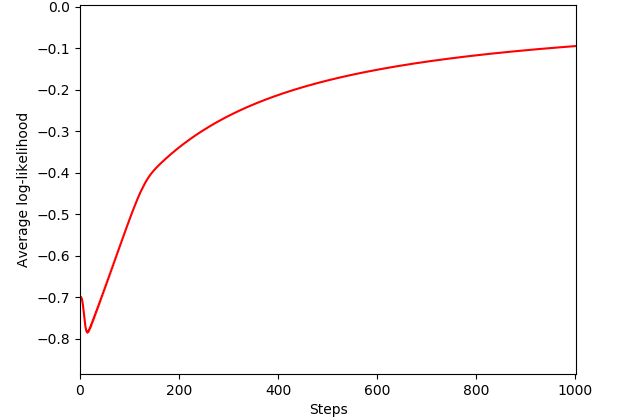
\includegraphics[width=\linewidth]{l=0-01log}
  \caption{Log-Likelihood being maximised when l = 0.01}
  \label{fig:T4}
\end{figure}

Learning rates of $\eta$ =[0.0001, 0.015, 0.011] for width's of l =[1, 0.1, 0.01] respectively. Smaller widths were more sensitive to oscillations about the maxima and no convergence. Convergence for the radial basis functions was slower than for a linear model, hence a smaller magnitude starting weight vector and more iterations were used. The likelihood plots for l=1 and 0.1 show that a maxima has been reached at the end of training. However in order to minimise over fitting and shorten training times the maxima wasn't reached when l=0.001. The likelihood on the training set with small widths can reach very high values, however this is because the weight vector's magnitude becomes very large as it learns almost exactly the training set. This exact learning reduced generality and success on an unseen test set.
%------------------------------------------------
\subsection{Probability contours}
Similarly to the linear case probability contours can be drawn for the three widths of RBF classifiers. These are shown in figures \ref{fig:c2} - \ref{fig:c4}.

\begin{figure}[h]
  \centering
    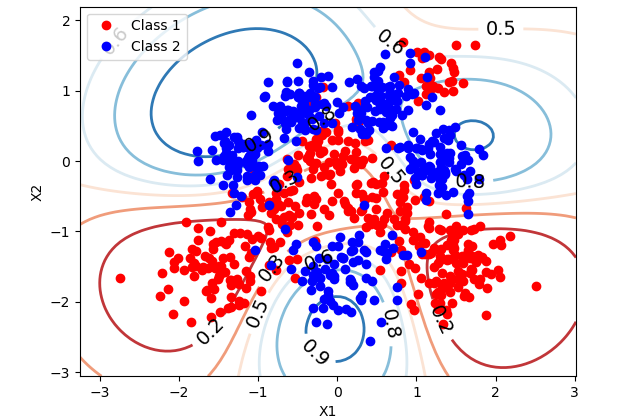
\includegraphics[width=\linewidth]{l=1contour}
  \caption{Probability contours of residing in the blue class for the RBF model of width 1}
  \label{fig:c2}
\end{figure}
\begin{figure}[h]
  \centering
    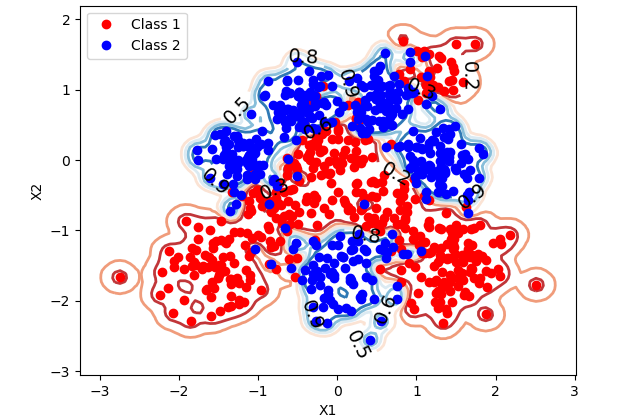
\includegraphics[width=\linewidth]{l=0-1contour}
  \caption{Probability contours of residing in the blue class for the RBF model of width 0.1}
  \label{fig:c3}
\end{figure}
\begin{figure}[h]
  \centering
    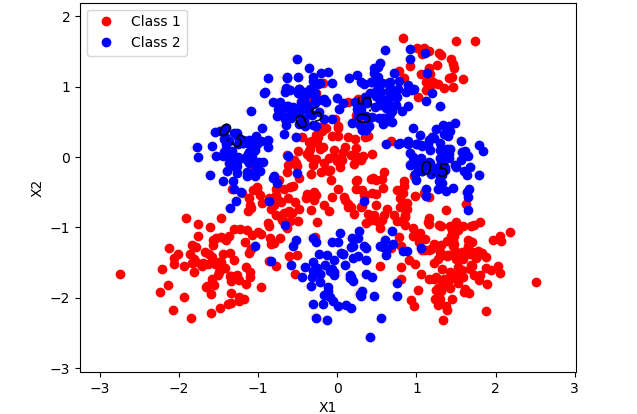
\includegraphics[width=\linewidth]{l=0-01contour}
  \caption{Probability contours of residing in the blue class for the RBF model of width 0.01}
  \label{fig:c4}
\end{figure}

figures \ref{fig:c2} - \ref{fig:c4} show that the width of RBF function is directly correlated to the proximity of the probability contours to the training data. With a large width of 1 the classes are separated well by the contours. However, the contours include large areas where no data was measured. This extrapolation could result in incorrect classification if the test data introduces a new cluster in a previously unseen region of the space $(x_1,x_2)$, a better estimate for unseen regions a probability nearer to 0.5. The adverse is true for small widths, the training has learnt where all the training points are and drawn small bubbles around them shown in figure \ref{fig:c5}. This causes over fitting and means classification of new points will mostly be wrong unless a test data point lies very close to a training point of the same class. Overfitting means any noise in the inputs will be likely to cause an incorrect classification. For this data the optimum width is between 0.1 and 1.
\begin{figure}[h]
  \centering
    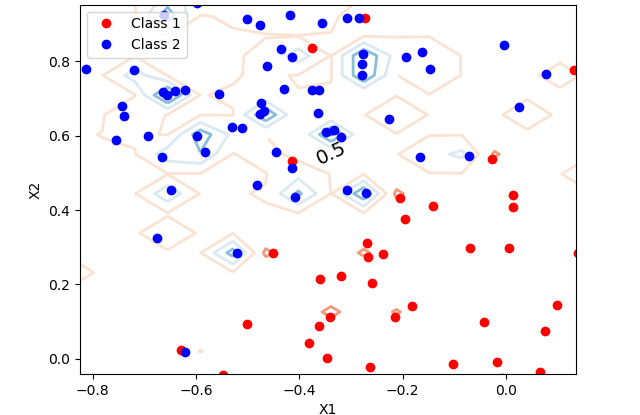
\includegraphics[width=\linewidth]{l=0-01contourzoom}
  \caption{Zoomed in probability contours of residing in the blue class for the RBF model of width 0.01}
  \label{fig:c5}
\end{figure}
%------------------------------------------------
\subsection{Confusion Matrix}
Confusion matrices can once again be calculated for the three RBF models in order to quantify performance. 
\newline 

\begin{center}
$\mathcal{C}_1=  
\begin{bmatrix}
    0.42 & 0.085  \\
    0.05 & 0.445 \\
\end{bmatrix}$

$\mathcal{C}_{0.1}=  
\begin{bmatrix}
    0.435 & 0.07  \\
    0.05 & 0.445 \\
\end{bmatrix}$

$\mathcal{C}_{0.01}=  
\begin{bmatrix}
    0.42 & 0.01  \\
    0.45 & 0.045 \\
\end{bmatrix}$
\end{center}

By looking at $\mathcal{C}_{0.01}$ it's shown that 87\% of test data is classified as class 1 (red). This is a result of the over fitting and causes very low success probability on the unseen test set. The classification becomes like a coin toss and is incorrect nearly 50\% of the time. Both $\mathcal{C}_{0.1}$ and $\mathcal{C}_1$ show a high success rate of 88\% and 86.5%. This is a large improvement on the linear classifier.
%------------------------------------------------
\onecolumn
\subsection{Log Likelihood per data point}
Additional comparisons between the four classifiers can be done by looking at the log-likelihood of each data point for the training and test sets. Figures \ref{fig:lltrain} and \ref{fig:lltrain} show these log-likelihoods on a scatter plot in order to gain a sense of magnitudes. To visualise the  log-likelihood with position in the data set see figures \ref{fig:lltrainmap} and \ref{fig:lltestmap}.
\begin{figure}[h]
  \centering
    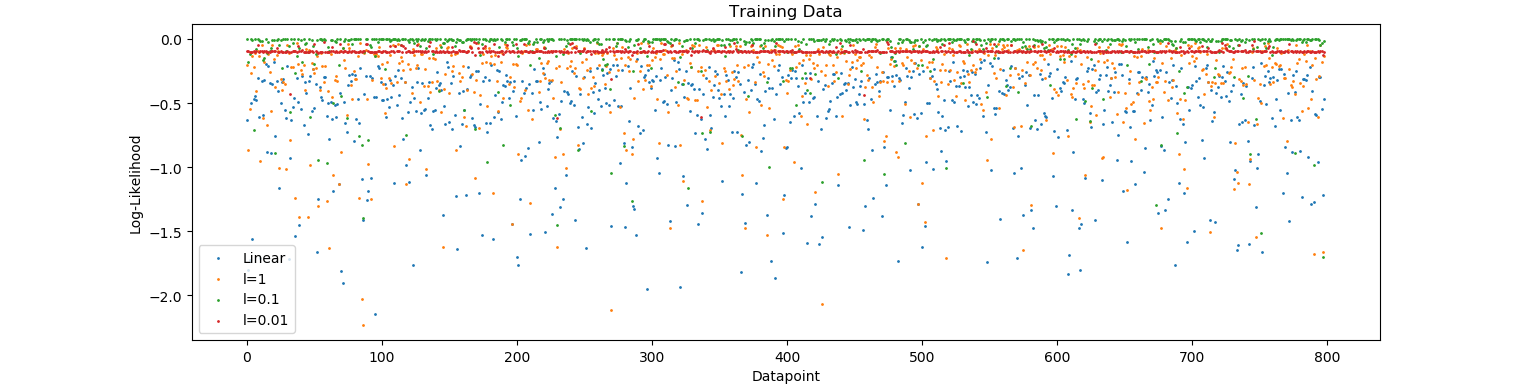
\includegraphics[width=\linewidth]{trainingdatall2}
  \caption{Plot of the log-likelihood for each datapoint in the training data set, for each of the four classifiers}
  \label{fig:lltrain}
\end{figure}
\begin{figure}[h]
  \centering
    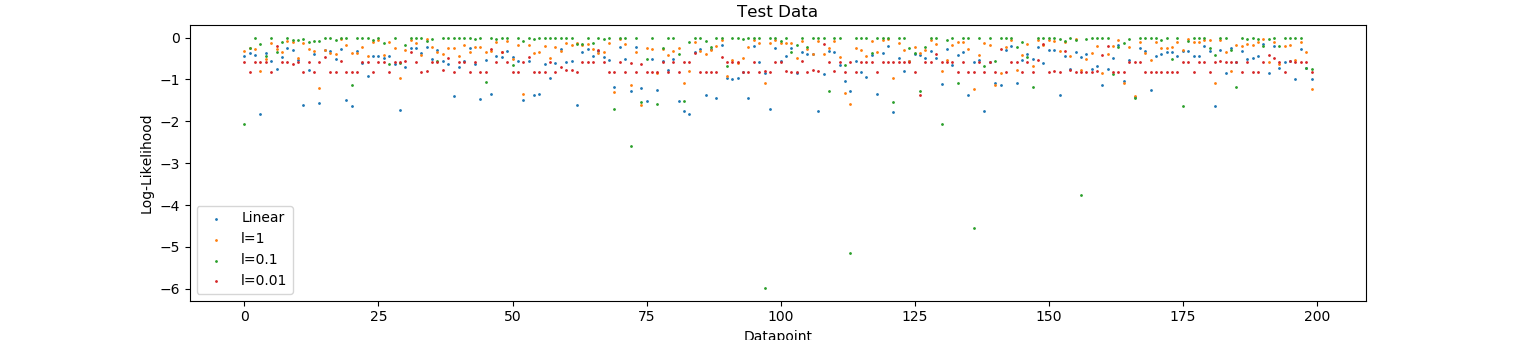
\includegraphics[width=\linewidth]{testdatall2}
  \caption{Plot of the log-likelihood for each datapoint in the test data set, for each of the four classifiers}
  \label{fig:lltest}
\end{figure}

Figure \ref{fig:lltrain} shows that all points in the training set for l=0.01 reach an almost constant likelihood. This is a sign of overfitting. For the test set the likelihood with l-0.01 is one of two values corresponding to the two classes, the likelihood is on general lower then the other classifiers. When l=0.1 the likelihood is lowest for the training data however large outliers appear on the test set due to data points in the test set residing slightly too far away from the observed training set. Both the linear classifier and RBF with l=1 show quite noisy log-likelihoods   possibly due to the larger sizes of region created.

\begin{figure}[h]
  \centering
    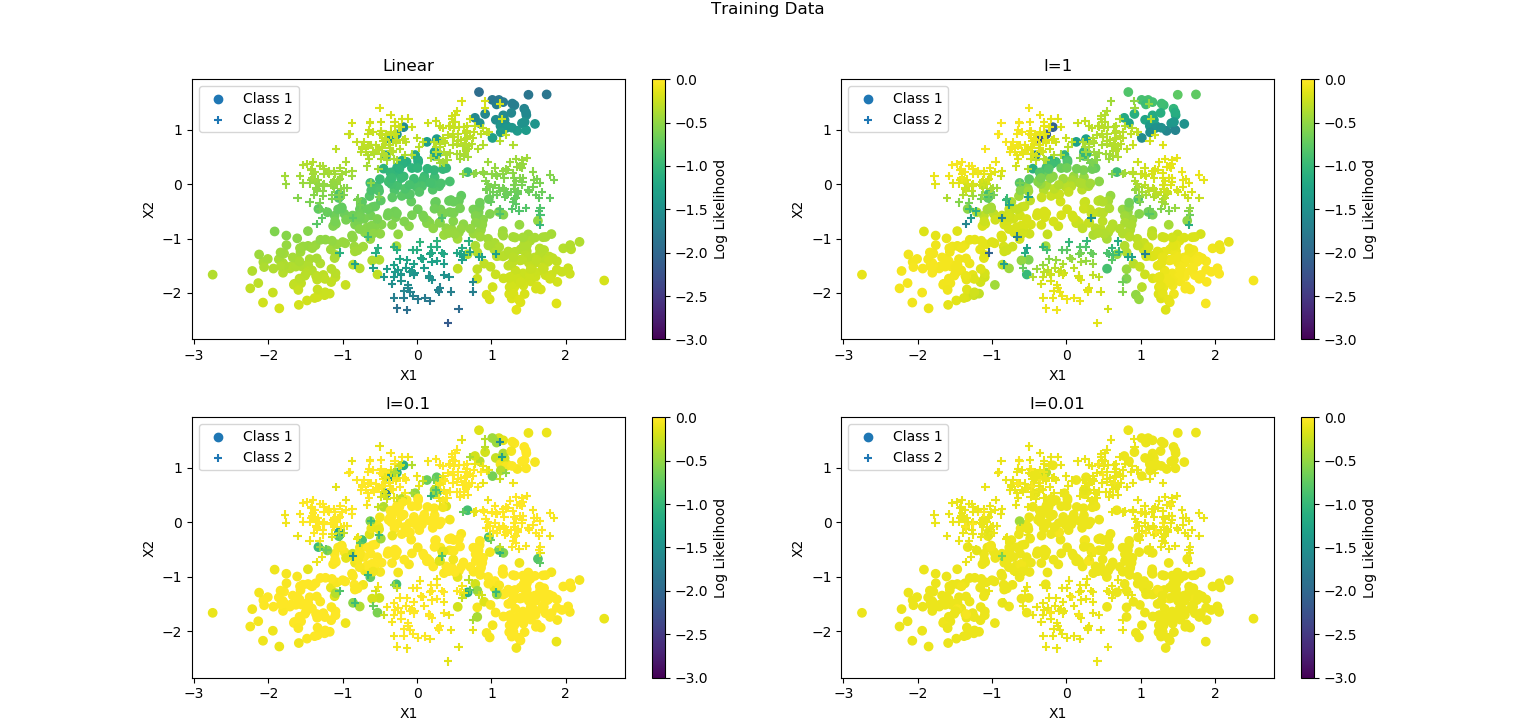
\includegraphics[width=\linewidth]{trainingdatallmap}
  \caption{Gradient plot showing the training log-likelihood for each classifier with the position in the data set}
  \label{fig:lltrainmap}
\end{figure}
\begin{figure}[h]
  \centering
    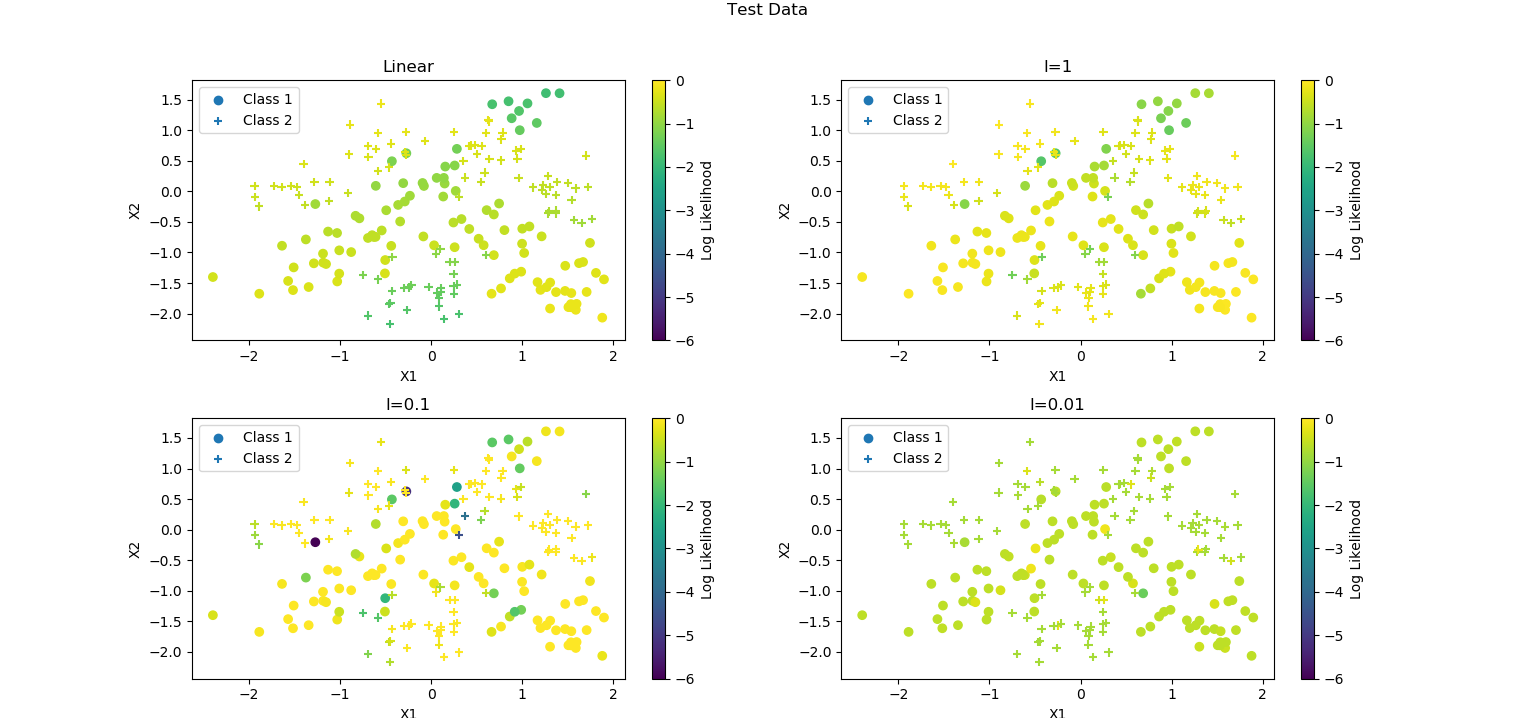
\includegraphics[width=\linewidth]{testdatallmap}
  \caption{Gradient plot showing the test log-likelihood for each classifier with the position in the data set}
  \label{fig:lltestmap}
\end{figure}

The same patterns can be seen by looking at the log-likelihoods with position. The RBF classifier with l=0.001 is a constant colour in the training set and two shades in the test set. The outliers when l=0.1 are shown to be on the edges of clusters of one group or when a data point of one class sits amongst lots of the other class. The more random nature of the linear and RBF with l=1 is shown to be due to certain groups in the $(x_1,x_2)$ space. Low likelihoods are assigned to any group on the incorrect side of the linear divide for the linear classifier. For l=0.1 these low likelihoods come from boundaries between cluster groups in particular the class 1 group at the top right, which in figure \ref{fig:c2} has class 2 probability contours running through.
\twocolumn
%----------------------------------------------------------------------------------------
\section{Appendix}
\subsection{1.1 Training Data}
\begin{lstlisting}
def gradient_ascent(beta,x_tilde,y):
    sigma = 1/(1+np.exp(-np.dot(x_tilde, beta))) # creates a vextor of sigma values
    gradient=np.matmul((y-sigma.T),x_tilde).T   #creates a gradient vector
    return beta + lrate*gradient

def train_data(X,y,beta,n):
    aveLike=np.zeros(n)
    for i in range(n):
        beta = gradient_ascent(beta,X,y)
        aveLike[i]=compute_average_ll(X,y,beta)
    plot_ll(aveLike)
    return beta
\end{lstlisting}
%-------------------------------------------------------   
\subsection{1.2 Computing Confusion Matrix}   
\begin{lstlisting}
def flip_numbers(x):
    return -x+1

def compute_confusion(testxtilde,testy,w):
    test_prob = logistic(np.dot(testxtilde, w))
    ytilde = test_prob //0.5
    confusion = np.array([[0,0],[0,0]])
    confusion[0,0] = np.dot(flip_numbers(testy),flip_numbers(ytilde)) # guess = 0 and value is 0
    confusion[0,1] = np.dot(flip_numbers(testy),ytilde) #guess = 1 , true = o
    confusion[1,0] = np.dot(testy,flip_numbers(ytilde))# guess = 0 , true value = 1
    confusion[1,1] = np.dot(testy,ytilde) #guess = 1 and true value = 1
    confusion = confusion / testy.shape[0]
    return confusion 
\end{lstlisting}
%------------------------------------------------
\end{document}
